\documentclass[tikz,border=10pt]{standalone}

\usepackage{float}
\usepackage{subfig}

\usepackage{framed}
\usepackage{listings}
\usepackage{graphicx}
\usepackage{textcomp}
\usepackage{tikz}
\usepackage{tikz-qtree}
\usetikzlibrary{shapes,automata,arrows}
\usepackage{pgfplots}
\usepackage{color}

\usetikzlibrary{calc,angles}
\usetikzlibrary{shapes,arrows,intersections}
\usetikzlibrary{matrix,fit,calc,trees,positioning,arrows,chains,shapes.geometric,shapes,angles}
\usetikzlibrary{quotes}

%\usetikzlibrary{calc,angles,quotes}
\tikzset{square/.style= { to path={ let \p1=(\tikztostart), \p2=(\tikztotarget),
  \p3=($(\p2)!1!90:(\p1)$), \p4=($(\p1)!1!-90:(\p2)$) in
  (\p2) foreach \i in {3,4,1,2} {--node[auto=right]{#1} (\p\i)}}}}



\usepackage{verbatim}


\begin{comment}

Hello
\end{comment}
\begin{document}

\newcommand{\pythagwidth}{3cm}
\newcommand{\pythagheight}{2cm}

\begin{tikzpicture}

  \coordinate [label={below right:$A$}] (A) at (0, 0);
  \coordinate [label={above right:$B$}] (B) at (0, \pythagheight);
  \coordinate [label={below left:$C$}] (C) at (-\pythagwidth, 0);

  \coordinate (D1) at (-\pythagheight, \pythagheight + \pythagwidth);
  \coordinate (D2) at (-\pythagheight - \pythagwidth, \pythagwidth);

  \draw [very thick] (A) -- (C) -- (B) -- (A);

 % \newcommand{\ranglesize}{0.3cm}
%  \draw (A) -- ++ (0, \ranglesize) -- ++ (-\ranglesize, 0) -- ++ (0, -\ranglesize);

 \draw (-0,0.5) arc (90:180:0.5cm);

  \draw [dashed] (A) -- node [below] {$b$} ++ (-\pythagwidth, 0)
            -- node [right] {$b$} ++ (0, -\pythagwidth)
            -- node [above] {$b$} ++ (\pythagwidth, 0)
            -- node [left] {$b$} ++ (0, \pythagwidth);

  \draw [dashed] (A) -- node [right] {$c$} ++ (0, \pythagheight)
            -- node [below] {$c$} ++ (\pythagheight, 0)
            -- node [left] {$c$} ++ (0, -\pythagheight)
            -- node [above] {$c$} ++ (-\pythagheight, 0);

  \draw [dashed] (C) -- node [above left] {$a$} (B)
                     -- node [below left] {$a$} (D1)
                     -- node [below right] {$a$} (D2)
                     -- node [above right] {$a$} (C);

\end{tikzpicture}


\tikz[thick] \draw (0,0) to[square=a] (0:3) to[square=b] ([turn]90:2) to[square=c] (0,0);


\begin{tikzpicture}
	\draw (-.5,0)--(1.5,0);
	\draw (0,-.5)--(0,1.5);

	\draw[] (0,0) -- (1,0) arc (0:90:1cm) -- cycle;
	\draw[]  (0.25,0.25) node[] {$\alpha$};
\end{tikzpicture}

\tikzset{
    a/.style={
        draw=green,
        line width=2pt,
        dashed,
    }
}

\begin{tikzpicture}[
	my angle/.style = {draw,
                   angle radius=7mm, 
                   angle eccentricity=1.1, 
                   right, inner sep=1pt,
                   font=\footnotesize} 
                   ]
\draw   
	(0,0) coordinate[label=below:$A$] (a) --
        (4,0) coordinate[label=below:$C$] (c) --
        (4,4) coordinate[label=above:$B$] (b) -- 
        cycle;
	
	\pic[draw=red, ->, angle eccentricity=1.2, angle radius=1cm] {angle=b--c--a};

	\pic[my angle] {angle = b--c--a};
	
	\draw [dashed] (4,4)  -- node[below] {a} node[above] {b} (8,4) -- (8,0) -- (4,0);            
\end{tikzpicture}


\begin{tikzpicture}[]
	\draw [dashed] (0,0)  -- ++(0,4) coordinate[label=above:$A$] -- ++(4,0) --  ++(0,-4)--  ++(-4,-0);
\end{tikzpicture}


\begin{tikzpicture}
	\draw (-.5,0)--(1.5,0);
	\draw (0,-.5)--(0,1.5);
\end{tikzpicture}

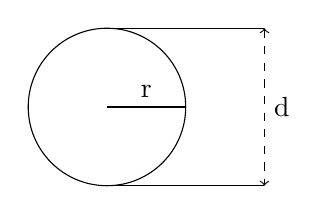
\begin{tikzpicture}
	\draw (0,0)--node[above] {r} (1,0);
	\draw (0,0) circle (1);
	\draw (0,-1)--(2,-1);
	\draw (0,+1)--(2,+1);
	\draw [dashed,<->] (2,1)--node[right] {d} (2,-1);
\end{tikzpicture}


\begin{tikzpicture}
\draw (0,0) -- (4,0) -- (4,4) -- (0,4) -- cycle;
\end{tikzpicture}


\begin{tikzpicture}

\draw (0,0) node{$\bullet$} node[left]{$O$};
\draw (0,0) circle(2cm);

\draw[->] (0,0)--(2.5,0) coordinate (X) node[right]{$x$};
\draw[->] (0,0)--(0,2.5) coordinate (Y) node[right]{$y$};

\draw ($(0,0)!2cm!(4,3)$) coordinate (P) node{$\bullet$} node[above right](P){$P$};


\end{tikzpicture}









\end{document}